%\documentclass[notes]{beamer}       % print frame + notes
%\documentclass[notes=only]{beamer}   % only notes
\documentclass{beamer}              % only frames
  \usepackage[english]{babel}
\usepackage[round]{natbib}
%\documentclass[hyperref={pdfpagelabels=false}]{beamer}
\usepackage{lmodern}
\usepackage{marvosym} % \MVRIGHTarrow

\usepackage{amsmath}  
\usepackage{multirow,graphicx,array}
\usepackage{multicol}
\usepackage{hhline}
\usepackage{xcolor}
\usepackage{colortbl}
\usepackage{threeparttable,booktabs}
\usepackage{chngcntr}
\usepackage{dcolumn}
\usepackage{caption}
\usepackage{fixltx2e}
\usepackage{rotating}
\usepackage{amssymb}



\usetheme{Singapore}
\useoutertheme{miniframes}
\AtBeginSection[]{\subsection{}}


\newcommand{\RowColor}{\rowcolor{gray} \cellcolor{white}}
\newcommand{\RowColorY}{\rowcolor{yellow} \cellcolor{white}}



\newcommand{\RN}[1]{%
  \textup{\uppercase\expandafter{\romannumeral#1}}%
}

\newcommand\Wider[2][3em]{%
\makebox[\linewidth][c]{%
  \begin{minipage}{\dimexpr\textwidth+#1\relax}
  \raggedright#2
  \end{minipage}%
  }%
}




\title{Effects of Weather on Maize Yield in Kenya}  
\author{Monika Novackova \\ \footnotesize supervised by: \textcolor{darkblue}{Pedram Rowhani, Martin Todd and Annemie Maertens}} 

\date{January 2019} 
\institute{University of Sussex}

\setbeamercolor{block title}{bg=purple!30,fg=black}





\begin{document}


\definecolor{LightCyan}{rgb}{0.88,1,1}
\definecolor{BeigeNadine}{rgb}{1,0.94,0.86}
\definecolor{DarkGreen}{rgb}{0.1803922,0.545098,0.3411765}
\definecolor{BeigeNadine}{rgb}{1,0.94,0.86}
\definecolor{PaleGreen}{rgb}{ 0.5960784,0.9843137, 0.5960784}
\definecolor{darkblue}{rgb}{0.0, 0.0, 0.55}
\definecolor{bored}{rgb}{0.8, 0.0, 0.0}
\definecolor{babypink}{rgb}{0.96, 0.76, 0.76}

 \newcolumntype{d}{D{.}{.}{-1}}
 \newcolumntype{e}{D{+}{\,\pm\,}{6,2}}




\maketitle


\normalsize

\begin{frame}
\frametitle{Outline}
\tableofcontents
\end{frame} 

\note{A}



\section{Introduction}


%oooooooooooooooooooooooooooooooooooooooooooooooooooooooooooooooooooooooooooooooooooooooooooooooooooooooooooooooooooooooooooooooooooooooooooooooooooooooooooooooooooooooooooooooooooo
%oooooooooooooooooooooooooooooooooooooooooooooooooooooooooooooooooooooooooooooooooooooooooooooooooooooooooooooooooooooooooooooooooooooooooooooooooooooooooooooooooooooooooooooooooooo

\begin{frame}\label{Introduction}
\frametitle{Introduction} 
 \begin{itemize}
\item SSRP project, related to ForPAc project
\item Extreme weather $\rightarrow$ disasters \textcolor{red}{(maybe name some years of drought in Kenya??)}

\begin{itemize}
\item Early warning systems have been developed
\end{itemize}
\item Goals: Improve early warning systems in Kenya
\item Shifting the disaster management from reactive to protective
\end{itemize} 

\begin{itemize}
\item Various approaches considered including:

\begin{itemize}
\item Relating NDMA Early warning phase classification to weather
\item Relating markets and food prices to weather
\item Relating maize yields to weather to weather
\item Computable general equilibrium (CGE) models
\end{itemize}
\end{itemize}
\end{frame}

\note{Climate change has been increasing amplitudes and frequency of extreme weather events\\ Not every hazard turns into disaster\\
Relating NDMA Early warning classification to weather also various precip and weather indexes
r
b}

%oooooooooooooooooooooooooooooooooooooooooooooooooooooooooooooooooooooooooooooooooooooooooooooooooooooooooooooooooooooooooooooooooooooooooooooooooooooooooooooooooooooooooooooooooooo
%oooooooooooooooooooooooooooooooooooooooooooooooooooooooooooooooooooooooooooooooooooooooooooooooooooooooooooooooooooooooooooooooooooooooooooooooooooooooooooooooooooooooooooooooooooo

\begin{frame}
       \hspace{-0.8cm}  \textbf{NDMA Early Warning Phase\\ \hspace{-0.8cm} Classification}
        
\vspace{-0.9cm}
     \begin{figure}
      \begin{columns}
        \column{.4\linewidth}
       
  \caption*{\textcolor{DarkGreen}{\textbf{\underline{\small{Example: Kitui county}}}}\\
   
 \vspace{0.25cm}\hspace{-0.25cm} \textbf{\textit{\textcolor{blue}{Normal $\rightarrow$ Alert $\rightarrow$  Alarm}}} \\
   \vspace{0.4cm}  
 \hspace{-0.25cm}  $\bullet$ \small{Bulletins for ASAL counties} \\
   \hspace{-0.25cm}  $\bullet$ \small{Online since 2013} \\
     \vspace{0.1cm}  
  \hspace{0.15cm}    \footnotesize{$\bullet$ But in pdf format} \\ 
    \vspace{0.1cm}  
\hspace{-0.25cm}   \small{$\bullet$ For county and month}
 
 }
        \column{.6\linewidth}

    \vspace{-0.16cm}   \hspace{-0.1cm}   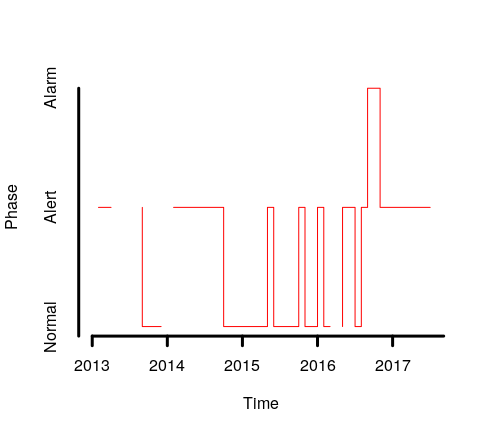
\includegraphics[width = 0.9\textwidth]{PhaseNA.png}  %565*238
 \vspace{-0.3cm}  
      \end{columns}
    \end{figure}
   
\vspace{-1.3cm}
    \begin{figure}
      \begin{columns}
        \column{.5\linewidth }

  \vspace{-1.8cm}        
        \column{.5\linewidth}
         
  \hspace{-2.6cm}  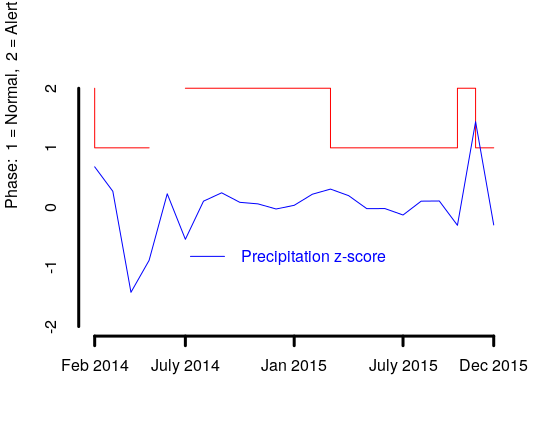
\includegraphics[width = 1.2\textwidth]{PrecNA.png}  %565*238
      \end{columns}
    \end{figure}

\end{frame}


\note{This is an example of one of the approaches that we eventually abandoned\\
b}




%oooooooooooooooooooooooooooooooooooooooooooooooooooooooooooooooooooooooooooooooooooooooooooooooooooooooooooooooooooooooooooooooooooooooooooooooooooooooooooooooooooooooooooooooooooo
%oooooooooooooooooooooooooooooooooooooooooooooooooooooooooooooooooooooooooooooooooooooooooooooooooooooooooooooooooooooooooooooooooooooooooooooooooooooooooooooooooooooooooooooooooooo


\begin{frame}\label{Approach}
\frametitle{Approach} 

\begin{itemize}
\item Narrowing the research question:
\begin{itemize}
\item Relationship of maize yield and weather in Kenya


\begin{itemize}
\item What is it about weather that causes drought related disasters?
\item Which particular characteristics of weather are the most 'responsible' for drought related disasters?
\end{itemize}
\end{itemize}
\end{itemize}

Sample:
\begin{itemize}
\item Panel of 47 counties of Kenya, $1981-2017$
\end{itemize}

\end{frame}

\note{After various problems with data (prices - not for every county, NDMA phases - not much of an objective criterion, probably political, various VCI values)
\\ so the decision about the approach was partially driven by data (un)availability}

%oooooooooooooooooooooooooooooooooooooooooooooooooooooooooooooooooooooooooooooooooooooooooooooooooooooooooooooooooooooooooooooooooooooooooooooooooooooooooooooooooooooooooooooooooooo
%oooooooooooooooooooooooooooooooooooooooooooooooooooooooooooooooooooooooooooooooooooooooooooooooooooooooooooooooooooooooooooooooooooooooooooooooooooooooooooooooooooooooooooooooooooo

\begin{frame}

\frametitle{Effects of droughts on economy}\label{Effects} 
\begin{block}{\textbf{Computable General Equilibrium (CGE)}}

\begin{itemize}

\item \underline{\textbf{\cite{robinson2010}}}
\begin{itemize}
\item 5 agro-ecological zones,46 production activities (incl. 35 zone specific agricultural production sectors), 22 commodity groups,  15 primary factors of production
\end{itemize}


\begin{table}
\begin{footnotesize}
\begin{tabular}{lll} 


\hline
\rowcolor{PaleGreen} \textbf{Fixed (inputs)} & \textbf{Determined by model (outputs)}  \\
 \hline
Capital stock& Domestic price of each commodity \\
Land (by region) & Land allocated across crops \\
Supply of labor per skill type& Real wages\\
Foreign capital inflow	& Real exchange rate\\
Trade balance	& \\
 \hline
\end{tabular}
\end{footnotesize}
\end{table}

\begin{footnotesize}

\item The simulation use a 'balanced' macro closure in which aggregate \textbf{investment, government demand, and consumption are fixed shares of total absorption}
\item Intermediate inputs into production are determined as fixed shares
of the quantity of output

\end{footnotesize}
\end{itemize}
\end{block}
\end{frame}
\note{

\vspace{0.3cm}
\vspace{0.3cm}a
\\
\vspace{0.3cm}a
\\
\vspace{0.3cm}a
}






\begin{frame}

\frametitle{Effects of droughts on economy}\label{Effects} 
\begin{block}{\textbf{Computable General Equilibrium (CGE)} Models }
\begin{itemize}




\item \underline{\textbf{\cite{OxfamIDS}}}
\begin{itemize}
\item Exploring range of scenarios for food price increase in 2030
\begin{itemize}
\item 1. Baseline 2. Climate change 3. Climate change with adaptation 4. Adaptation only in sub-Saharan Africa
\end{itemize}
\item Global coverage, set of individual country models, linked through international trade
\item Climate change (incl. drought) modelled as changes in factor productivity (usually negative)

\end{itemize}

\end{itemize}
\end{block}
\end{frame}



\note{A}


























\section{My Suggestion}


\begin{frame}

\frametitle{My suggestion - panel estimation}\label{MySuggestion1} 

My interest: \textbf{Effects of drought on economy in Kenya}
\begin{itemize}

\item \textbf{Response variable}

\begin{itemize}
\item Volumes of production (crop specific, total)
\item Profit per acre \normalsize{\citep{Deschenes2007Ric}}

\begin{itemize}
\item \footnotesize{(Value of agricultural products - prod. expanses)/acres (crops, pasture, grazing)}\\ 
\end{itemize}
\end{itemize}
\item \textbf{Units of analysis}
\begin{itemize}
\item Counties in Kenya $\times$ year
\
\end{itemize}


\item \textbf{Explanatory variable of interest}

\begin{itemize}
\item Dummy variable (0/1) drought occurred in a particular county and year or not
\item Several varieties - various specifications of drought:

\end{itemize}


\end{itemize}

\end{frame}






\note{also I can try some t-tests, f-test for various grouping - WHAT WOULD BE THE BEST DEFFINITION OF DROUGHT year x county\\
\vspace{0.3cm}a\\
\vspace{0.3cm}}

















\begin{frame}

\frametitle{My idea - panel estimation}\label{MySuggestion4} 


\begin{align*}
\begin{array}{lcl}
 Y_{i,t} &=& \alpha_i +\gamma_t + \delta D'_{i,t} +  \boldsymbol{\beta X_{i,t}}+ \epsilon_{i,t}
\end{array}
\end{align*}

\begin{table}
\begin{small}
\begin{tabular}{lll}

$Y_{i,t}$ &$=$& Response variable (food production/price), county $i$ in year $t$\\
$\alpha_i$ &$=$& Fixed effects, county $i$\\
{\color{darkblue}$\delta$ }&{\color{darkblue}$=$}&{\color{darkblue}{Effect of drought on economy}}\\
$D_{i,t}$ &$=$& Indicator variable\\
& &  $D=1$ if drought in county $i$ in year $t$, $D=0$ otherwise\\
$\boldsymbol{\beta}$ &$=$& Vector of effects of other covariates\\
$X_{i,t}$ &$=$& Matrix of values of other covariates in county $i$ in year $t$\\
$\epsilon_{i,t}$ &$=$& Error term \\
{\color{DarkGreen}$\gamma_t$} & {\color{DarkGreen}$=$}& {\color{DarkGreen}Year specific indicator?}
\end{tabular}
\end{small}
\end{table}

\end{frame}


\note{Also waldtest, jako ekvivalent pro celkovy f-test byl signifikantni>> overall fit je moc o}



\note{hello}


\section*{}

\frame[allowframebreaks]{ 
\centering
\huge{Thank you for attention}
}

\note{hello}

\frame[allowframebreaks]{ 
\small
\frametitle{References}
\bibliographystyle{apa}
\bibliography{referencesFS}
}

\end{document}

